\documentclass[12pt]{article}
\usepackage[a4paper, total={6in, 10in}]{geometry}
\usepackage{graphicx}
\graphicspath{{figs/}} 


\title{Demonstration of Human-Humanoid Collaboration} 
\author{Miguel Xochicale and Chris Baber \\ 
School of Engineering \\
University of Birmingham
}
\date{November 2018}

\begin{document}
\maketitle
%\thispagestyle{empty} %No number


\begin{abstract}
Technical report for the demonstration of a human-humanoid collaboration 
activity at the Open Day at The University of Birmingham.
\end{abstract}

\section{Introduction}
For the demo, NAO, a humanoid robot \cite{gouaillier2008} has been programmed 
to move their arms from left to right in a continues way (Fig \ref{fig:nao}).




%%---------------------------------(FIGURE)-------------------------------------
\begin{figure}[ht]
\centering
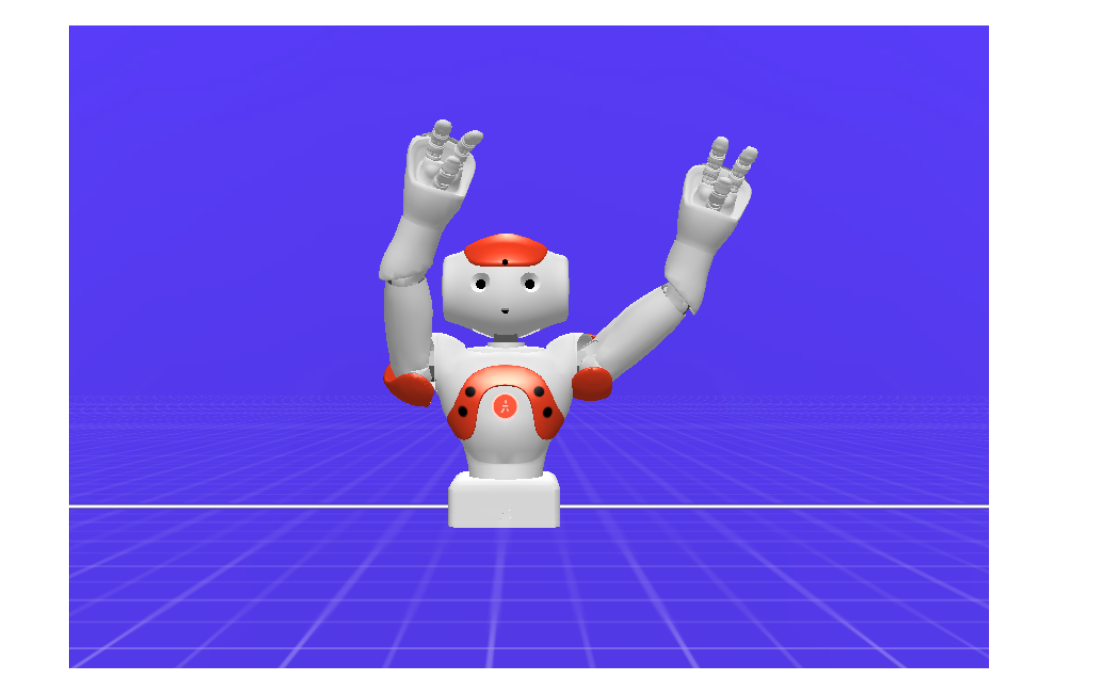
\includegraphics[width=0.5\textwidth]{nao/naoarms}
    \caption{
	{\bf Nao.}
	 Upper arm movements of NAO.
        }
\label{fig:nao}
\end{figure}
%%---------------------------------(FIGURE)------



\section{Setting up}

%%---------------------------------(FIGURE)-------------------------------------
\begin{figure}[ht]
\centering
\includegraphics[width=0.5\textwidth]{experiment/setup/setup}
    \caption{
	{\bf Setting up of experiment.}
	(A) A rectangular box is put in front of NAO,  
	(B) the distance is approximately 8 cm considering the 
	both the box and the base of NAO are at the same height.
        }
\label{fig:st}
\end{figure}
%%---------------------------------(FIGURE)------





\section{Effects of Lights with Colours}
Adquiring pictures with different light conditions
make changes of the filtered images.
It requires more investigation to tackle light 
dependencies to tackle better such problem.
It can also be raised a question regarding the consideration
of different skin colours of users when interaction with NAO.


Particularly, the reflection of light in the bricks
which make detecting less of the surface area, as well
as the use of certain colour. Green colour is hardly 
detected when using only artificial light, but 
using blue brick is a bit better, however there is 
some problems with the light reflectance that 
show a bit of white colour. Fig. \ref{fig:bbp}.

%%---------------------------------(FIGURE)-------------------------------------
\begin{figure}[ht]
\centering
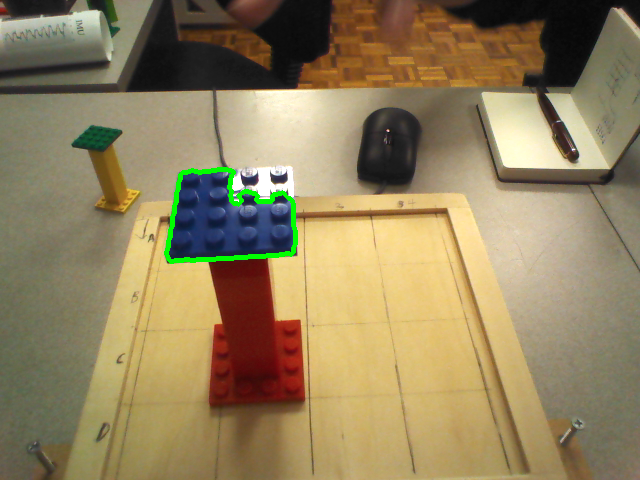
\includegraphics[width=0.5\textwidth]{experiment/bricks/bluebrickproblem}
    \caption{
	{\bf Blue colour detection with OpenCV.}
	Problem with detection of colours with OpenCV \cite{opencv_library}
	for reflection of light in the bricks.
        }
\label{fig:bbp}
\end{figure}
%%---------------------------------(FIGURE)------





\newpage

\bibliographystyle{apalike}
\bibliography{references/references}


\end{document}
